% === Cours de Java
% === Chapitre : Introduction

\subsection{Concepts}

\imgfullw{../img/coffeemug.jpg}{
	\Large\textbf{\color{white}programmer}\\
	\textit{\color{gray}[proh-gram-er]}\\
	{\large\color{white}an organism that turn caffeine into software}
}{https://www.flickr.com/photos/secret_canadian/22234285/sizes/o/}

\begin{frame}{D�finitions}
D�finissons les concepts suivants :
\begin{itemize}
\item Un \emph{programme} ?
\item \emph{Programmer} ?
\item Un \emph{langage de programmation} ? 
\item Diff�rence entre \emph{langue} et \textit{langage} ?
\end{itemize}
\end{frame}


\begin{frame}{Un programme}
La seule chose dont est capable un ordinateur est de r�aliser extr�mement rapidement des instructions �l�mentaires
\par\bigskip
Toute t�che qu'on veut lui confier doit donc �tre pr�alablement d�crite comme une suite s�quentielle d'instructions (un programme)
\note[item]{\url{http://en.wikipedia.org/wiki/Source_lines_of_code} donne des exemples de taille de programmes}
\end{frame}



\begin{frame}{Un langage}
\emph{Une classe de langages est adapt�e � une classe de probl�mes \dots\ et ces probl�mes �voluent dans le temps \dots}
\note[item]{On peut aborder ici l'historique des langages : machine, assembleur, haut niveau, structur�, orient� objet, fonctionnels, orient�s aspects\dots}
\end{frame}


\subsection{Traduction}

\begin{frame}{Le probl�me de la traduction}
Un ordinateur ne comprend que le langage machine. N�cessit� d'une \emph{traduction}
\bigskip
\begin{center}
\begin{tabular}{c|c}
\emph{Compilation} & \emph{Interpr�tation} \\ \hline
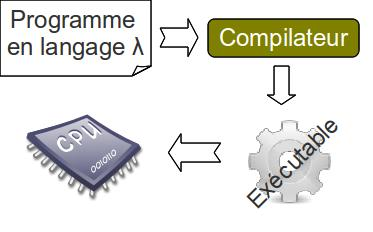
\includegraphics[scale=.35]{../img/java-jvm-compil} &
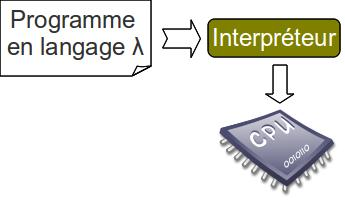
\includegraphics[scale=.35]{../img/java-jvm-interp} \\
\textit{\small traduit d'une traite} & \textit{\small traduit morceau par morceau} \\
\textit{\small avant l'ex�cution} & \textit{\small au moment de l'ex�cution} \\
\end{tabular} 
\end{center}
\note[item]{Faire une comparaison des avantages/inconv�nients}
\end{frame}

\full[bluepigment]{
	\begin{center}
		\color{white}
		{\huge\bf Et \sigle{Java} ?}
		\bigskip\\
		{\large Compil� ou interpr�t� ?}
	\end{center}
}


